%% FullCourse_10Lecs -- Lecture 8, Act 8.3 (RETRIEVE): Vector Search and GraphRAG.
%% Rebuilt 2026-07-08 per Lec08_Rewrite_Plan_2026-07-08.md ("one map, five acts").
%% Source: archive_pre_split/pre_map_rebuild_2026-07-08/Lec08_T3_Vector_Retrieval_GraphRAG.tex
%% (26 frames -> 15; ANN internals and the RRF formula reduced to intuition,
%% re-ranking folded into the hybrid frame, GraphRAG block compressed 17 -> 7
%% frames around the GRAM case study; systems snapshots/benchmarks/future cut).

%% Shared preamble for the FullCourse_10Lecs topic decks.
%%
%% Each topic .tex \input's this file, then defines its own \title, \date
%% override (if any), \graphicspath, and \begin{document}.
%%
%% Reconstructed verbatim from the inlined copy preserved in
%% Lec10_Case_Studies/Lec10_T8_Case6_DeepRamsey.tex (lines 23-190), which is
%% explicitly annotated there as "from ../shared_preamble.tex, copied verbatim".
%% Base preamble matches MiniCourse_8hr/Slides/shared_preamble.tex; this version
%% additionally provides \sectiondivider, the conceptbox/cautionbox/examplebox/
%% takeawaybox tcolorboxes, and \compacttables used across the split decks.

\documentclass[10pt,english,aspectratio=169]{beamer}

\usepackage{ae,aecompl}
\usepackage[T1]{fontenc}
\usepackage{textcomp}
\usepackage[utf8]{inputenc}
\usepackage{babel}
\usepackage{datetime2}

\setcounter{secnumdepth}{3}
\setcounter{tocdepth}{3}

\usepackage{amsmath, amssymb, amsthm, graphicx}
\usepackage{booktabs, multirow}
\usepackage{tikz}
\usepackage{pgfplots}
\pgfplotsset{compat=1.16}
\usepackage[most]{tcolorbox}
\tcbuselibrary{skins, breakable, theorems}
\usepackage{listings}
\usepackage{xcolor}

\lstset{
  basicstyle=\ttfamily\small,
  keywordstyle=\color{blue!80!black}\bfseries,
  commentstyle=\color{green!50!black}\itshape,
  stringstyle=\color{orange!80!black},
  backgroundcolor=\color{gray!8},
  frame=single,
  rulecolor=\color{gray!40},
  breaklines=true,
  showstringspaces=false,
  numbers=none,
}

\lstdefinestyle{pythonstyle}{
    language=Python,
    basicstyle=\ttfamily\footnotesize,
    keywordstyle=\color{blue!80!black}\bfseries,
    commentstyle=\color{green!50!black}\itshape,
    stringstyle=\color{orange!80!black},
    frame=single,
    breaklines=true,
    showstringspaces=false,
    numbers=left,
    numbersep=5pt,
    numberstyle=\tiny\color{gray},
    backgroundcolor=\color{gray!8},
    rulecolor=\color{gray!40}
}

\ifx\hypersetup\undefined
  \AtBeginDocument{%
    \hypersetup{bookmarks=false,breaklinks=true,pdfborder={0 0 0},colorlinks=true,
      linkcolor=DarkText,urlcolor=RedTitle}%
  }
\else
  \hypersetup{bookmarks=false,breaklinks=true,pdfborder={0 0 0},colorlinks=true,
    linkcolor=DarkText,urlcolor=RedTitle}%
\fi

\makeatletter
\newcommand\makebeamertitle{%
  \begin{frame}[plain]
    \vspace*{1.0cm}
    \centering
    {\usebeamerfont{title}\usebeamercolor[fg]{title}\inserttitle\par}
    \vspace{1.0cm}
    {\usebeamerfont{author}\usebeamercolor[fg]{author}\insertauthor\par}
    \vspace{0.2cm}
    {\usebeamerfont{date}\usebeamercolor[fg]{date}\insertdate\par}
  \end{frame}}%
\AtBeginDocument{%
  \let\origtableofcontents=\tableofcontents
  \def\tableofcontents{\@ifnextchar[{\origtableofcontents}{\gobbletableofcontents}}
  \def\gobbletableofcontents#1{\origtableofcontents}%
}

\usetheme{metropolis}
\usefonttheme{professionalfonts}

\definecolor{LightGray}{RGB}{230,230,230}
\definecolor{RedTitle}{RGB}{0,0,200}
\definecolor{VeryLightGray}{RGB}{245,245,245}
\definecolor{DarkText}{RGB}{0,0,0}

\setbeamercolor{background canvas}{bg=white}
\setbeamercolor{title}{fg=RedTitle}
\setbeamercolor{author}{fg=DarkText}
\setbeamercolor{date}{fg=DarkText}
\setbeamercolor{frametitle}{bg=VeryLightGray,fg=DarkText}
\setbeamercolor{normal text}{fg=DarkText}
\setbeamerfont{title}{size=\large}

\setbeamersize{text margin left=5mm, text margin right=5mm}
\addtobeamertemplate{frametitle}{}{\vspace{-0.5em}}
\newcommand{\reducevspace}{\vspace{-0.5cm}}

% Shared section divider and box styles for split topic decks.
\newcommand{\sectiondivider}[2]{%
\begin{frame}[plain,noframenumbering]
\begin{center}
\vfill
{\Large\textbf{#1}\par}
\vspace{0.35cm}
{\normalsize #2\par}
\vfill
\end{center}
\end{frame}
}

\newtcolorbox{conceptbox}[1][]{
  colback=blue!3,
  colframe=RedTitle!55,
  boxrule=0.35mm,
  arc=1mm,
  left=2mm,
  right=2mm,
  top=1mm,
  bottom=1mm,
  #1
}
\newtcolorbox{cautionbox}[1][]{
  colback=red!3,
  colframe=red!50!black,
  boxrule=0.35mm,
  arc=1mm,
  left=2mm,
  right=2mm,
  top=1mm,
  bottom=1mm,
  #1
}
\newtcolorbox{examplebox}[1][]{
  colback=green!3,
  colframe=green!45!black,
  boxrule=0.35mm,
  arc=1mm,
  left=2mm,
  right=2mm,
  top=1mm,
  bottom=1mm,
  #1
}
\newtcolorbox{takeawaybox}[1][]{
  colback=VeryLightGray,
  colframe=RedTitle!55,
  boxrule=0.35mm,
  arc=1mm,
  left=2mm,
  right=2mm,
  top=1mm,
  bottom=1mm,
  #1
}
\newcommand{\compacttables}{\renewcommand{\arraystretch}{1.15}}

\setbeamertemplate{navigation symbols}{}
\setbeamertemplate{footline}{%
  \hfill%
  \usebeamercolor[fg]{page number in head/foot}%
  \usebeamerfont{page number in head/foot}%
  \insertframenumber\,/\,\inserttotalframenumber\kern1em\vskip2pt%
}

\makeatother

\author{Zhigang Feng}
% "date with time": compile timestamp so each build is identifiable.
\date{\today\ \DTMcurrenttime}

\metroset{sectionpage=none}

\usetikzlibrary{arrows.meta, positioning, shapes, shapes.geometric, fit, calc, backgrounds}

% Macros for the GRAM four-mechanism diagram (ported from the instructor's
% research deck). \providecommand so nothing clashes with shared_preamble.tex.
\providecommand{\OLG}{OLG}
\providecommand{\LLM}{\textsc{llm}}
\providecommand{\RAG}{\textsc{rag}}
\providecommand{\GraphRAG}{\textsc{GraphRAG}}

\graphicspath{{./pic/}{./figures/}{../../MiniCourse_8hr/Slides/Module4_Agentic_AI/pic/}{../}}

%% Lec08 shared MAP slide: "one map, five acts" recurring diagram.
%% Adapted from ../Lec07_LLM/lec07_map.tex (\LecSevenMap -> \LecEightMap).
%% Input this file AFTER ../shared_preamble.tex (needs RedTitle, VeryLightGray)
%% and call \LecEightMap{k} inside a frame, where k in {1..5} highlights the
%% current act ("you are here") and k = 0 renders the closing reprise with all
%% five acts complete (used by T5's closing frame).
%% Filename deliberately does not match the build glob Lec*_T*.tex, so the
%% build script never tries to compile it standalone.

\newcommand{\LecEightMap}[1]{%
% Precompute per-box style selectors; TikZ option lists are comma-split before
% TeX conditionals run, so \ifnum must not sit inside a [...] options list.
\ifnum#1=0
  \tikzset{lecmapa/.style={lecmapdone}, lecmapb/.style={lecmapdone},
           lecmapc/.style={lecmapdone}, lecmapd/.style={lecmapdone},
           lecmape/.style={lecmapdone}}%
\else
  \tikzset{lecmapa/.style={}, lecmapb/.style={}, lecmapc/.style={},
           lecmapd/.style={}, lecmape/.style={}}%
  \ifnum#1=1 \tikzset{lecmapa/.style={lecmapcur}}\fi
  \ifnum#1=2 \tikzset{lecmapb/.style={lecmapcur}}\fi
  \ifnum#1=3 \tikzset{lecmapc/.style={lecmapcur}}\fi
  \ifnum#1=4 \tikzset{lecmapd/.style={lecmapcur}}\fi
  \ifnum#1=5 \tikzset{lecmape/.style={lecmapcur}}\fi
\fi
\begin{center}
\begin{tikzpicture}[
    act/.style={rectangle, rounded corners, draw=black!60, fill=VeryLightGray,
        minimum width=2.6cm, minimum height=0.92cm, text width=2.5cm,
        align=center, font=\scriptsize, text=DarkText},
    lecmapcur/.style={draw=RedTitle, very thick, fill=orange!20},
    lecmapdone/.style={draw=green!45!black, thick, fill=green!10},
    q/.style={font=\tiny\itshape, text width=2.7cm, align=center, text=black!70},
    sat/.style={rectangle, rounded corners, draw=black!45, dashed, fill=white,
        text width=5.0cm, align=center, font=\tiny, text=black!70,
        minimum height=0.5cm},
    barlab/.style={font=\tiny\bfseries, text=black!60},
    arr/.style={-{Stealth[length=2mm]}, thick, gray!60}
]
    % --- five act boxes ---
    \node[act, lecmapa] (a1) at (0,0)
        {\textbf{8.1 WALL}\\ \tiny naive prompting fails};
    \node[act, lecmapb] (a2) at (2.85,0)
        {\textbf{8.2 INDEX}\\ \tiny chunk \& embed once};
    \node[act, lecmapc] (a3) at (5.7,0)
        {\textbf{8.3 RETRIEVE}\\ \tiny vector, hybrid, graph};
    \node[act, lecmapd] (a4) at (8.55,0)
        {\textbf{8.4 GENERATE}\\ \tiny cited, refusable answers};
    \node[act, lecmape] (a5) at (11.4,0)
        {\textbf{8.5 APPLY}\\ \tiny corpora, demo, evaluation};
    \draw[arr] (a1) -- (a2);
    \draw[arr] (a2) -- (a3);
    \draw[arr] (a3) -- (a4);
    \draw[arr] (a4) -- (a5);
    % --- the student question each act answers ---
    \node[q] at (0,-0.82)    {why not just paste\\ it all in?};
    \node[q] at (2.85,-0.82) {how does my corpus\\ become searchable?};
    \node[q] at (5.7,-0.82)  {how does the right\\ passage come back?};
    \node[q] at (8.55,-0.82) {how do I get citations,\\ not hallucinations?};
    \node[q] at (11.4,-0.82) {what does this change\\ for my research?};
    % --- "you are here" marker above the current act ---
    \ifnum#1=1 \node[font=\scriptsize\bfseries, text=RedTitle] at (0,0.95)
        {you are here\ $\blacktriangledown$};\fi
    \ifnum#1=2 \node[font=\scriptsize\bfseries, text=RedTitle] at (2.85,0.95)
        {you are here\ $\blacktriangledown$};\fi
    \ifnum#1=3 \node[font=\scriptsize\bfseries, text=RedTitle] at (5.7,0.95)
        {you are here\ $\blacktriangledown$};\fi
    \ifnum#1=4 \node[font=\scriptsize\bfseries, text=RedTitle] at (8.55,0.95)
        {you are here\ $\blacktriangledown$};\fi
    \ifnum#1=5 \node[font=\scriptsize\bfseries, text=RedTitle] at (11.4,0.95)
        {you are here\ $\blacktriangledown$};\fi
    \ifnum#1=0 \node[font=\scriptsize\bfseries, text=green!45!black] at (5.7,0.95)
        {all five acts complete};\fi
    % --- bottom band: problem / pipeline / payoff ---
    \fill[blue!10]   (-1.3,-1.55) rectangle (1.40,-1.22);
    \fill[green!10]  (1.65,-1.55) rectangle (9.85,-1.22);
    \fill[orange!15] (10.1,-1.55) rectangle (12.7,-1.22);
    \node[barlab] at (0.05,-1.385) {THE PROBLEM};
    \node[barlab] at (5.75,-1.385) {THE PIPELINE};
    \node[barlab] at (11.4,-1.385) {YOUR RESEARCH};
    % --- the recurring spine (the RAG pipeline), printed under the band ---
    \node[font=\tiny\itshape, text=black!60] at (5.7,-1.83)
        {the pipeline:\ \ corpus $\to$ chunk $\to$ embed $\to$ index
         \;$\big\|$\; query $\to$ retrieve $\to$ augment $\to$ cited answer};
    % --- dashed satellites: the neighbouring lectures ---
    \node[sat] at (2.0,-2.42)
        {\textit{before 8.1:} Lec07 gave you the language engine --- frozen
         weights, finite context; RAG is its grounded memory};
    \node[sat] at (9.8,-2.42)
        {\textit{after 8.5:} Lec09 agents --- retrieval becomes one tool the
         model chooses to call $\to$ Lec10 cases};
\end{tikzpicture}
\end{center}
}


\title[AI for Econ Research]{AI for Economic Research: Dynamic Models, Language, and Agents\\
Lecture 8.3: Retrieve --- Vector Search and GraphRAG}

\begin{document}

\makebeamertitle

%=============================================================================
\begin{frame}{Map: Act 8.3 --- Bring the Right Passage Back}
\textbf{The index exists; this act is the online lookup --- and what to do when similarity alone is not enough.}
\LecEightMap{3}
\textit{\footnotesize Route this deck: vector search in practice $\to$ where similarity fails $\to$ GraphRAG and the GRAM case study.
Thread A: filter FOMC chunks by date and type, then query them; Thread B: the OLG literature becomes a typed graph.}
\end{frame}

%=============================================================================
\section{Vector Search in Practice}
\sectiondivider{Vector Search in Practice}{From similarity math to a working index}

\begin{frame}{Why a Vector Database?}
\textbf{Millions of chunks now carry 1024-dim vectors --- where do they live?}

\medskip
\begin{itemize}
\item \textbf{The naive option:} a flat numpy array on disk; search by computing similarity to every vector and sorting.
\begin{itemize}
    \item Works fine for $10{,}000$ vectors; at $1{,}000{,}000$ a query takes seconds; at $10{,}000{,}000$ it is impractical.
    \item No metadata filters. No incremental updates. No persistence.
\end{itemize}

\medskip
\item \textbf{A vector database} solves all four:
\begin{enumerate}
    \item \emph{Scale:} approximate nearest-neighbor search over millions of vectors in milliseconds.
    \item \emph{Metadata filters:} restrict search to ``date $\geq$ 2020 AND doc\_type = minutes.''
    \item \emph{Incremental updates:} add new chunks as documents arrive, without rebuilding.
    \item \emph{Persistence:} the index lives on disk and survives restarts.
\end{enumerate}
\end{itemize}
\end{frame}

\begin{frame}{Similarity Search 101 --- and Why Approximate}
\textbf{Retrieval is nearest-neighbor search: given a query vector $q$, find the $K$ closest chunk vectors $d_i$.}

\medskip
\begin{itemize}
\item \textbf{Three common similarity functions:} cosine $\;\cos(\theta) = \frac{q \cdot d_i}{\|q\| \, \|d_i\|}$; \; dot product $\;q \cdot d_i$; \; (negative) Euclidean distance $\;-\|q - d_i\|$.

\medskip
\item \textbf{Why cosine is the default:} it ignores vector length. Modern embedders L2-normalize their outputs, so cosine $=$ dot product: \emph{higher dot product $\Rightarrow$ more similar}. Geometrically: each chunk is an arrow from the origin; cosine measures the \emph{angle} to the query arrow.

\medskip
\item \textbf{Why approximate?} Exact search touches every vector: $10^7$ vectors $\times$ 1024 dims $\approx 10^{10}$ operations \emph{per query} --- seconds of latency.

\medskip
\item \textbf{ANN (approximate nearest neighbor):} trade $\sim$1\% of recall for orders-of-magnitude speedups. Names to recognize when you read the docs: \textbf{HNSW} (graph walks) and \textbf{IVF} (cluster, then search the nearest cells). In practice \emph{your vector DB picks the default} --- you won't tune this by hand.
\end{itemize}
\end{frame}

\begin{frame}{Vector DB Landscape: Scale vs.\ Hosting}
\begin{center}
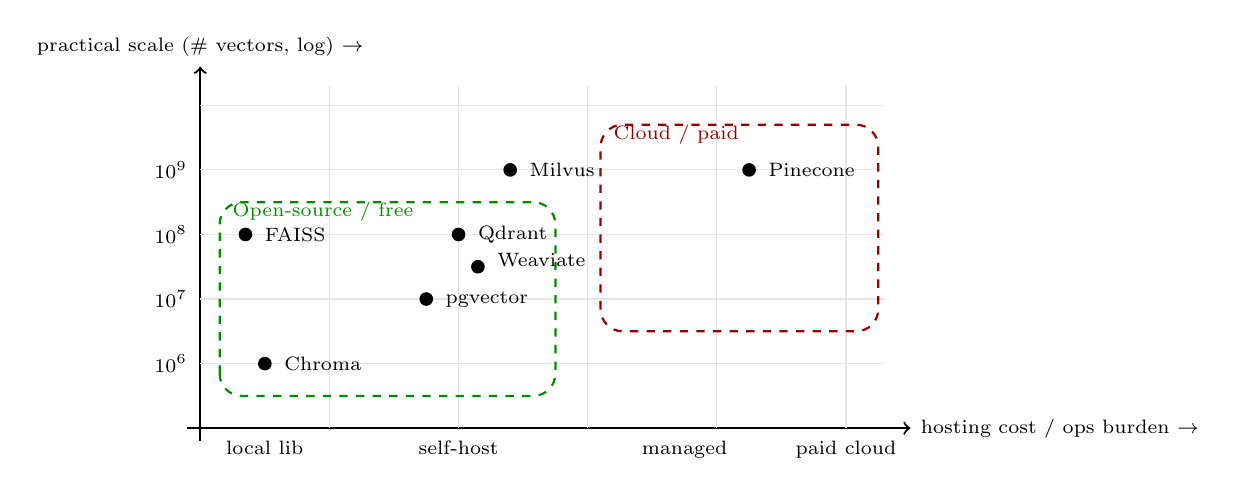
\begin{tikzpicture}[font=\footnotesize, scale=0.82]
  % axes
  \draw[->, thick] (-0.2,0) -- (11.0,0) node[right, font=\scriptsize] {hosting cost / ops burden $\to$};
  \draw[->, thick] (0,-0.2) -- (0,5.6) node[above, font=\scriptsize] {practical scale (\# vectors, log) $\to$};
  % grid
  \foreach \y in {1,2,3,4,5} \draw[gray!20] (0,\y) -- (10.6,\y);
  \foreach \x in {2,4,6,8,10} \draw[gray!20] (\x,0) -- (\x,5.3);

  % y-axis labels
  \node[font=\scriptsize, anchor=east] at (-0.05,1) {$10^6$};
  \node[font=\scriptsize, anchor=east] at (-0.05,2) {$10^7$};
  \node[font=\scriptsize, anchor=east] at (-0.05,3) {$10^8$};
  \node[font=\scriptsize, anchor=east] at (-0.05,4) {$10^9$};
  % x-axis labels
  \node[font=\scriptsize, anchor=north] at (1.0,-0.05) {local lib};
  \node[font=\scriptsize, anchor=north] at (4.0,-0.05) {self-host};
  \node[font=\scriptsize, anchor=north] at (7.5,-0.05) {managed};
  \node[font=\scriptsize, anchor=north] at (10.0,-0.05) {paid cloud};

  % Open-source box
  \draw[draw=green!55!black, thick, dashed, rounded corners=8pt]
       (0.3,0.5) rectangle (5.5,3.5);
  \node[green!55!black, font=\scriptsize, anchor=south west] at (0.35,3.05) {Open-source / free};

  % Cloud / paid box
  \draw[draw=red!60!black, thick, dashed, rounded corners=8pt]
       (6.2,1.5) rectangle (10.5,4.7);
  \node[red!60!black, font=\scriptsize, anchor=south west] at (6.25,4.25) {Cloud / paid};

  % Systems as dots
  \fill[black] (0.7,3.0) circle (3pt); \node[font=\scriptsize, anchor=west] at (0.85,3.0) {FAISS};
  \fill[black] (1.0,1.0) circle (3pt); \node[font=\scriptsize, anchor=west] at (1.15,1.0) {Chroma};
  \fill[black] (4.0,3.0) circle (3pt); \node[font=\scriptsize, anchor=west] at (4.15,3.0) {Qdrant};
  \fill[black] (4.3,2.5) circle (3pt); \node[font=\scriptsize, anchor=west] at (4.45,2.6) {Weaviate};
  \fill[black] (4.8,4.0) circle (3pt); \node[font=\scriptsize, anchor=west] at (4.95,4.0) {Milvus};
  \fill[black] (3.5,2.0) circle (3pt); \node[font=\scriptsize, anchor=west] at (3.65,2.0) {pgvector};
  \fill[black] (8.5,4.0) circle (3pt); \node[font=\scriptsize, anchor=west] at (8.65,4.0) {Pinecone};
\end{tikzpicture}
\end{center}

\smallskip
\textbf{For an economist starting out:} \textbf{Chroma} or \textbf{FAISS} for laptop/cluster work (free, local, simple); \textbf{pgvector} if you already run Postgres (reuses existing infra); \textbf{Pinecone / Qdrant cloud} if you need a hosted index and have budget.
\end{frame}

\begin{frame}{Hybrid Retrieval, Plus a Light Re-Rank}
\textbf{Dense retrieval finds meanings, not strings --- so production systems pair it with a keyword engine and a re-ranking pass.}

\smallskip
\begin{itemize}
\item \textbf{The dense-only failure case:} \emph{``find every speech mentioning Section 13(3)''} --- a precise legal-citation query. Embeddings cluster similar \emph{meanings}, not similar \emph{strings}; the top-10 neighbors discuss the discount window in general, not the section.

\smallskip
\item \textbf{The fix --- hybrid:} also run a classical sparse retriever in parallel. \textbf{BM25} (TF-IDF-based) scores exact term matches, catching rare strings, acronyms, statute citations, tickers. Merging the two ranked lists is a solved problem (\emph{rank fusion}) that your library implements.

\smallskip
\item \textbf{A light re-rank on top:} the fast bi-encoder returns a top-50 shortlist; a \emph{cross-encoder} then reads query and candidate \emph{together} and reorders --- top-5 in, much sharper relevance out. Open default: \texttt{bge-reranker-large}.
\end{itemize}

\smallskip
\begin{takeawaybox}
Hybrid dense+sparse (+ re-rank) is the \textbf{production default} (mid-2026). Pure dense is rarely competitive.
\end{takeawaybox}
\end{frame}

\begin{frame}{Metadata Filters}
\textbf{Research queries carry \emph{structural} constraints that pure semantic search cannot express.}

\smallskip
\begin{itemize}
\item \textbf{Real example:} \emph{``Find all FOMC discussions of unemployment from 2020 onwards, excluding press conferences.''}
\begin{itemize}
    \item ``Discussions of unemployment'' $\Rightarrow$ semantic search.
    \item ``From 2020 onwards'' $\Rightarrow$ filter on \texttt{date $\geq$ 2020-01-01}.
    \item ``Excluding press conferences'' $\Rightarrow$ filter on \texttt{doc\_type $\neq$ press\_conference}.
\end{itemize}
Modern vector DBs combine similarity with SQL-style filters in a single query.

\smallskip
\item \textbf{This is exactly why preserving rich metadata at chunking time matters} (the Act 8.2 gotcha). If chunks don't carry \texttt{date}, \texttt{doc\_type}, \texttt{speaker}, you cannot filter on them later.
\end{itemize}

\smallskip
\begin{takeawaybox}
\textbf{Rule of thumb:} add \emph{more} metadata than you think you need. It is cheap at index time and impossible to reconstruct after the fact.
\end{takeawaybox}
\end{frame}

\begin{frame}[fragile]{Code: Build a Chroma Index and Query It}
\begin{lstlisting}[language=Python, basicstyle=\ttfamily\footnotesize]
import chromadb
from sentence_transformers import SentenceTransformer

model = SentenceTransformer("BAAI/bge-large-en-v1.5")
client = chromadb.PersistentClient(path="./fomc_index")  # on disk
coll = client.get_or_create_collection("fomc")

# Add chunks with embeddings + metadata
coll.add(
    ids=[f"chunk_{i}" for i in range(len(chunks))],
    documents=chunks,
    embeddings=model.encode(chunks, normalize_embeddings=True).tolist(),
    metadatas=[{"meeting": "2024-06", "doc_type": "minutes"} for _ in chunks],
)

# Query with a metadata filter
q = model.encode(["How did the Committee discuss inflation?"],
                 normalize_embeddings=True).tolist()
results = coll.query(query_embeddings=q, n_results=5,
                     where={"doc_type": "minutes"})
\end{lstlisting}
\end{frame}

%=============================================================================
\section{When Similarity Is Not Enough}
\sectiondivider{When Similarity Is Not Enough}{Relationship questions need edges, not echoes}

\begin{frame}{Where Vanilla Vector RAG Starts to Break}
\textbf{Dense retrieval is a local similarity machine --- strong on lookup, blind to structure.}

\medskip
\begin{itemize}
\item It misses three important structures:
\begin{enumerate}
    \item \textbf{Relationships between objects.} Two chunks may matter because their entities are \emph{linked}, even if the wording differs.
    \item \textbf{Global structure.} Nearest-neighbor search has no notion of themes, camps, or argument clusters across an entire corpus.
    \item \textbf{Coverage.} If the same fact appears in many chunks, top-$K$ retrieval returns duplicates instead of a representative overview.
\end{enumerate}

\medskip
\item \textbf{Economist examples:}
\begin{itemize}
    \item ``Which Senators most often connect inflation to housing supply constraints?''
    \item ``What are the main camps in recent papers on LLMs and education?''
\end{itemize}

\medskip
\item Once the question is \textbf{multi-hop} or \textbf{corpus-level}, plain top-$K$ chunk retrieval is often the wrong abstraction.
\end{itemize}
\end{frame}

\begin{frame}{Concrete Break Point: The Phillips-Curve Question}
\textbf{Question:} \emph{``Which Phillips-curve papers use survey expectations and are cited by post-2020 FOMC speeches?''}

\smallskip
\begin{columns}[T,totalwidth=\textwidth]
\column{0.49\textwidth}
\textbf{Vanilla vector RAG}
\begin{itemize}\small
\item Embeds the query as one vector.
\item Returns 5 chunks that \emph{sound like} ``Phillips curve + survey expectations.''
\item Has \textbf{no notion of citation edges} between NBER papers and FOMC speeches.
\item Best case: a chunk that \emph{discusses} both topics, even if no citation link exists.
\item Failure mode: confident, fluent, but the cited link is fictional.
\end{itemize}

\column{0.49\textwidth}
\textbf{GraphRAG}
\begin{itemize}\small
\item Walks the citation graph: NBER paper $\to$ \texttt{cited\_by} edge $\to$ FOMC speech node.
\item Filters by node attribute: \texttt{date $\geq$ 2020}.
\item Filters by paper attribute: \texttt{uses\_data: SurveyOfProfessionalForecasters}.
\item Returns the actual subgraph; only then generates from the supporting chunks.
\item Failure mode: degrades to ``no path found,'' not invention.
\end{itemize}
\end{columns}

\vspace{0.12cm}
\begin{takeawaybox}
\textbf{Rule:} reach for GraphRAG when the question is \emph{about a relationship}, not just \emph{about a topic}. Top-$K$ similarity cannot manufacture an edge that the index does not represent.
\end{takeawaybox}
\end{frame}

\begin{frame}{Knowledge Graphs: Adding Structure to Retrieval}
\begin{columns}[T,totalwidth=\textwidth]
\column{0.50\textwidth}
\begin{itemize}
\item A \textbf{knowledge graph (KG)} stores facts as \textbf{nodes + edges} rather than isolated chunks.

\medskip
\item Canonical form: \texttt{<head, relation, tail>} --- e.g.\ \texttt{<Powell, discusses, inflation expectations>}, or across papers: \texttt{<Paper B, cites, Paper A>}.

\medskip
\item \textbf{Build/use:} offline, extract entities and relations (optionally summarize communities); online, retrieve the \emph{relevant subgraph} --- entity nodes, chunk nodes, community summaries.

\medskip
\item The gain: retrieval is no longer ``find text that sounds similar'' --- it can \emph{follow links}.
\end{itemize}

\column{0.46\textwidth}
\centering
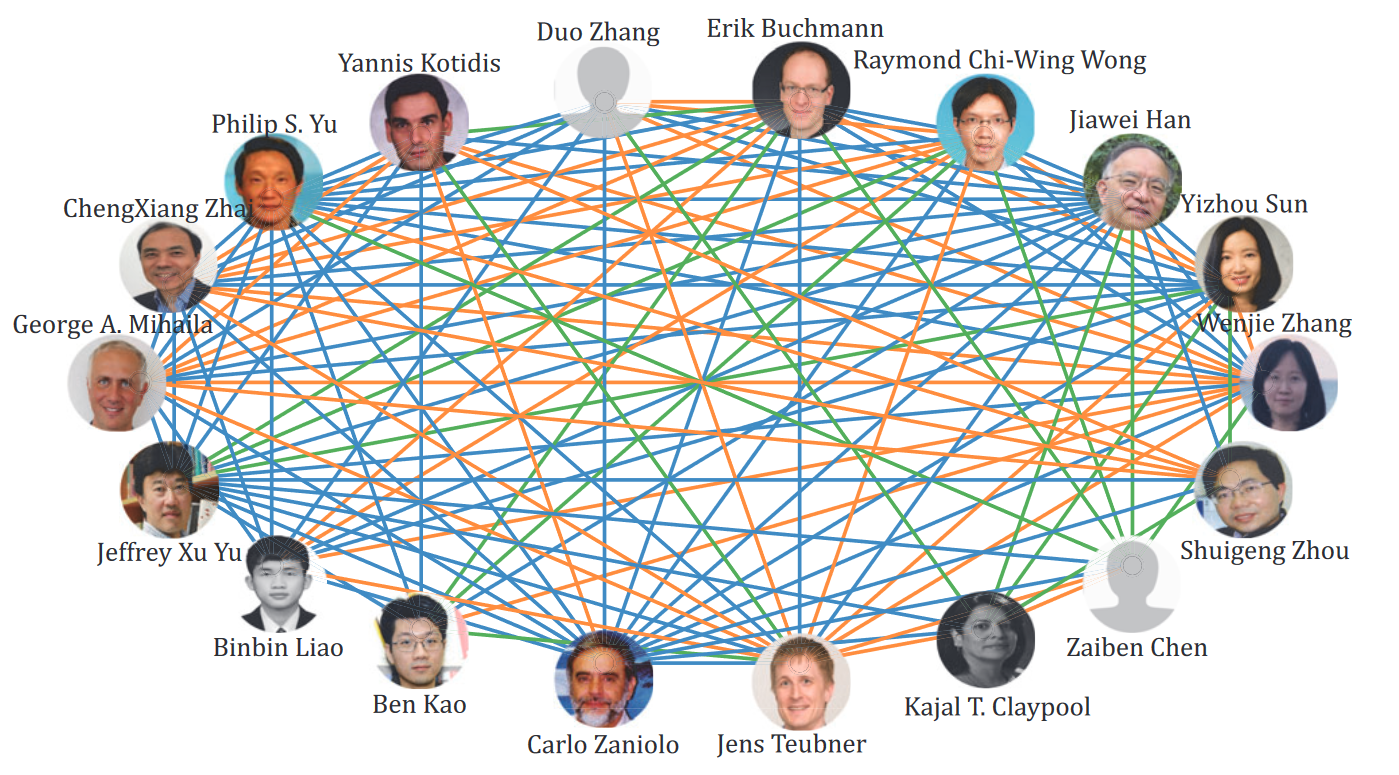
\includegraphics[width=\linewidth]{graph_rag_share/knowledge_graph_example.png}

\scriptsize
Once facts are stored as a graph, retrieval can follow links rather than isolated paragraphs.
\end{columns}
\end{frame}

\begin{frame}{Vanilla RAG vs.\ GraphRAG: A Direct Comparison}
\textbf{Match the retrieval architecture to the question type --- neither dominates everywhere.}

\medskip
\begin{center}
\footnotesize
\begin{tabular}{|p{3.2cm}|p{4.6cm}|p{5.2cm}|}
\hline
\textbf{Question type} & \textbf{Vector / hybrid RAG} & \textbf{GraphRAG} \\ \hline
Specific fact lookup & Strong when the exact chunk is nearby & Strong if fact is attached to an entity or path \\ \hline
Relationship query & Often requires several retrieved chunks and luck & Natural: traverse edges and retrieve neighborhoods \\ \hline
Global summarization & Top-$K$ chunks under-cover the corpus & Community reports summarize modules of the corpus \\ \hline
High redundancy corpus & May retrieve near-duplicate boilerplate & Can collapse repeated facts into entities/communities \\ \hline
Cost and complexity & Simpler, cheaper, easier to debug & More expensive offline; KG quality matters \\ \hline
\end{tabular}
\end{center}

\medskip
\textbf{Research rule:} start with vector + BM25 + re-rank. Move to graph retrieval \emph{only} when the question requires relationships or corpus-level themes you can't get from local similarity.
\end{frame}

\begin{frame}{Case Study: GRAM --- Four Mechanisms on One OLG Query}
\textbf{The instructor's own GRAM: a domain-typed GraphRAG over a curated 157-paper OLG corpus --- the research-grade sibling of the Act 8.5 demo.}

\smallskip
\footnotesize\itshape
``\OLG{} life-cycle, idiosyncratic $+$ aggregate shocks, incomplete intergenerational asset markets --- which solver class is admissible for the joint stationary distribution in recursive equilibrium?''
\normalfont
\begin{center}
\resizebox{!}{0.50\textheight}{%
\begin{tikzpicture}[
  font=\footnotesize,
  node distance=2.4mm,
  q/.style       ={draw,rounded corners=1pt,inner sep=2pt,minimum width=20mm,minimum height=4.5mm,fill=gray!5},
  corpus/.style  ={draw,rounded corners=0.5pt,inner sep=2pt,minimum width=20mm,minimum height=4.5mm,fill=red!10,align=center},
  pasted/.style  ={draw,rounded corners=0.5pt,inner sep=2pt,minimum width=20mm,minimum height=4.5mm,fill=yellow!22,align=center},
  vdb/.style     ={cylinder,shape border rotate=90,draw,aspect=0.22,minimum width=20mm,minimum height=11mm,fill=gray!18,font=\footnotesize,align=center,inner sep=1pt},
  kgicon/.style  ={draw,rounded corners=1pt,inner sep=2pt,minimum width=20mm,minimum height=11mm,fill=green!14,align=center},
  ctx/.style     ={draw,rounded corners=1pt,inner sep=1.5pt,minimum width=20mm,minimum height=4.5mm,fill=yellow!25,font=\scriptsize\itshape,align=center},
  llm/.style     ={draw,rounded corners=1pt,inner sep=2pt,minimum width=20mm,minimum height=4.5mm,fill=blue!14,align=center},
  ans/.style     ={draw,rounded corners=1pt,inner sep=2pt,minimum width=20mm,minimum height=4.5mm,fill=gray!5,align=center},
  outcome/.style ={text width=24mm,align=center,font=\scriptsize\itshape,text=gray!50!black},
  arr/.style     ={-{Latex[length=1.5mm]},semithick},
  hdr/.style     ={font=\footnotesize\bfseries,align=center,text width=24mm},
  gnode/.style   ={circle,inner sep=0pt,minimum size=1.2mm,fill=green!60!black}
]
\node[hdr] (h1) at (0,0) {Naive\\\LLM};
\node[q,below=of h1] (q1) {query};
\node[llm,below=of q1] (l1) {\LLM};
\node[ans,below=of l1] (a1) {answer};
\node[outcome,below=1mm of a1] {silent\\structural failure};
\draw[arr] (q1) -- (l1); \draw[arr] (l1) -- (a1);

\node[hdr] (h2) at (2.85,0) {In-context\\stuffing};
\node[pasted,below=of h2] (cp2) {pasted\\excerpts};
\node[ctx,below=4mm of cp2] (ctx2) {query + pasted text};
\node[llm,below=of ctx2] (l2) {\LLM};
\node[ans,below=of l2] (a2) {answer};
\node[outcome,below=1mm of a2] {bounded by\\user curation};
\draw[arr] (cp2) -- (ctx2); \draw[arr] (ctx2) -- (l2); \draw[arr] (l2) -- (a2);

\node[hdr] (h3) at (5.7,0) {\RAG\\(embedding)};
\node[corpus,below=of h3] (cp3) {literature};
\node[vdb,below=4mm of cp3] (vdb3) {embeddings};
\node[ctx,below=4mm of vdb3] (ctx3) {query + top-$k$\\passages};
\node[llm,below=of ctx3] (l3) {\LLM};
\node[ans,below=of l3] (a3) {answer};
\node[outcome,below=1mm of a3] {wrong-by-prominence};
\draw[arr] (cp3) -- (vdb3); \draw[arr] (vdb3) -- (ctx3); \draw[arr] (ctx3) -- (l3); \draw[arr] (l3) -- (a3);

\node[hdr] (h4) at (8.55,0) {\GraphRAG\\(GRAM)};
\node[corpus,below=of h4] (cp4) {literature};
\node[kgicon,below=of cp4] (kg4) {};
\node[font=\scriptsize] at ($(kg4.north)+(0,-1.6mm)$) {typed graph};
\node[gnode] (g1) at ($(kg4.center)+(-4mm,-2mm)$) {};
\node[gnode] (g2) at ($(kg4.center)+(0mm,-2.5mm)$) {};
\node[gnode] (g3) at ($(kg4.center)+(4mm,-2mm)$) {};
\node[gnode] (g4) at ($(kg4.center)+(-2mm,0.3mm)$) {};
\node[gnode] (g5) at ($(kg4.center)+(2mm,0.3mm)$) {};
\draw[gray!55,thin] (g1)--(g2) (g2)--(g3) (g4)--(g2) (g5)--(g2) (g1)--(g4) (g3)--(g5);
\node[ctx,below=of kg4] (ctx4) {query + ranked\\subgraph};
\node[llm,below=of ctx4] (l4) {\LLM};
\node[ans,below=of l4] (a4) {cited\\answer};
\node[outcome,below=1mm of a4,text=green!45!black] {ranked $+$\\condition-aware};
\draw[arr] (cp4) -- (kg4); \draw[arr] (kg4) -- (ctx4); \draw[arr] (ctx4) -- (l4); \draw[arr] (l4) -- (a4);
\end{tikzpicture}}
\end{center}

\smallskip
\textit{\footnotesize Why economics is special: every paper is math \emph{and} prose --- math is analysis, prose is mechanism. An econ assistant needs both; GRAM sits between math-IR and legal/clinical RAG.}
\end{frame}

\begin{frame}{Wrong-by-Prominence vs.\ Condition-Aware Retrieval}
\begin{itemize}
\item \textbf{Wrong-by-prominence:} pure embedding retrieval routes the query to the \emph{most prominent} paper, whether or not it fits the asked-for conditions:
\begin{itemize}\small
    \item ``OLG with capital'' $\Rightarrow$ Diamond (1965), \emph{not} Auerbach--Kotlikoff (1987).
    \item ``heterogeneous-agent macro'' $\Rightarrow$ Aiyagari, \emph{not} Krusell--Smith.
\end{itemize}
\emph{The vocabulary is present; the applicability filter is absent.}

\smallskip
\item \textbf{Condition-aware:} admissibility is \emph{conditional} --- add aggregate risk and a different solver class becomes admissible. Embedding similarity cannot encode that dependency; a walk over a \emph{typed} graph of model objects can.

\smallskip
\item \textbf{Two corpus lessons worth copying:} a non-trivial \emph{post-cutoff share} (RAG demonstrably adds value); \emph{citation connectivity} (unlinked documents are unreachable).
\end{itemize}

\smallskip
\begin{takeawaybox}
\textbf{Honest framing.} These labels name each mechanism's \emph{failure mode} on this query type. GRAM's condition-aware advantage is the \textbf{gap a planned three-condition evaluation (naive / RAG / GraphRAG) is designed to measure} --- a design goal, not yet a reported win; one in-progress, unpublished pipeline.
\end{takeawaybox}
\end{frame}

\begin{frame}{Choosing the Retrieval Architecture}
\begin{center}
\renewcommand{\arraystretch}{1.15}
\small
\begin{tabular}{|p{3.2cm}|p{3.1cm}|p{5.8cm}|}
\hline
\textbf{Question type} & \textbf{Best first choice} & \textbf{Why} \\
\hline
Precise factual lookup or citation hunt & Hybrid dense + sparse RAG & Exact strings, dates, and citations matter more than global structure. \\
\hline
Specific multi-hop entity question & Graph-based RAG & The answer depends on linked entities and paths rather than one chunk. \\
\hline
Broad summarization over a large corpus & Graph / hierarchical retrieval & You need coverage of themes, not just the closest paragraphs. \\
\hline
Fast prototype on a changing corpus & Vanilla RAG first & A flat vector index is easy to build and update; add structure only if it buys accuracy. \\
\hline
\end{tabular}
\end{center}

\medskip
\textbf{Rule of thumb:} start with hybrid dense+sparse. Escalate to graph retrieval when the task requires \emph{relationships}, \emph{coverage}, or \emph{multi-hop reasoning}.

\smallskip
\textit{\footnotesize Names to recognize in this space: Microsoft GraphRAG, LightRAG, HippoRAG, RAPTOR --- Edge et al.\ (2024); Guo et al.\ (2024); Guti\'errez et al.\ (2024); Sarthi et al.\ (2024).}
\end{frame}

\begin{frame}{Bridge: The Right Passage Is Back --- Now Answer From It}
\textbf{Act 3 delivered the online lookup: hybrid vector+keyword search with metadata filters as the default, graph retrieval when the question is about relationships.}

\medskip
\begin{itemize}
\item The GRAM case shows where this is heading for research corpora: typed structure over the literature, so retrieval respects \emph{conditions}, not just vocabulary.

\medskip
\item Eventually an \emph{agent} will choose vector vs.\ graph vs.\ web search itself --- Act 8.5 closes on that bridge to Lecture 9.

\medskip
\item \textbf{Next --- Act 8.4 (GENERATE):} retrieved chunks are not an answer yet. The generation contract: a prompt template that grounds, cites, and \emph{refuses} --- plus the decision matrix against fine-tuning.
\end{itemize}

\bigskip
\centering
\footnotesize\textit{Arc: Act 1 WALL $\to$ Act 2 INDEX $\to$ \textbf{Act 3 RETRIEVE} $\to$ Act 4 GENERATE $\to$ Act 5 APPLY.}
\end{frame}

\end{document}
